\documentclass[tikz, border=10pt]{standalone}
\usepackage{pgfplots}
\usepgfplotslibrary{groupplots}
\pgfplotsset{compat=1.18}

\begin{document}
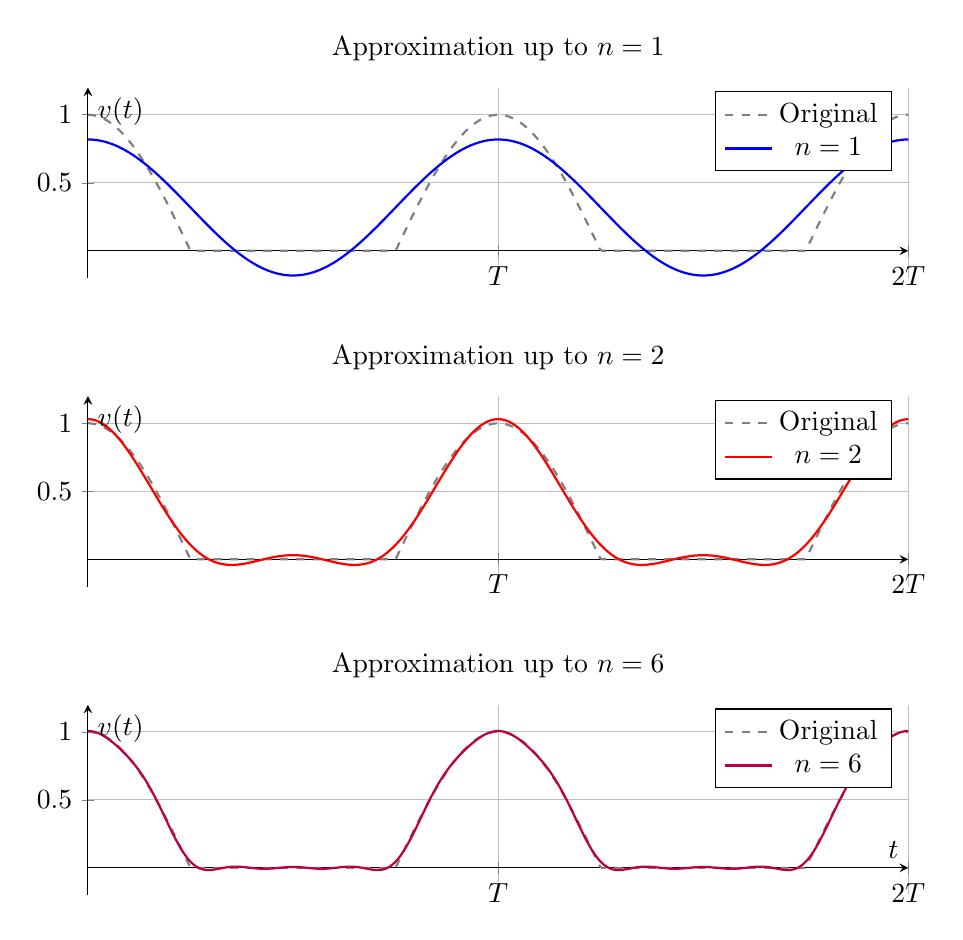
\begin{tikzpicture}
    \begin{groupplot}[
        group style={
            group size=1 by 3,
            vertical sep=1.5cm,
            xlabels at=edge bottom
        },
        width=12cm, height=4cm,
        axis lines=middle,
        xlabel={$t$}, ylabel={$v(t)$},
        ymin=-0.2, ymax=1.2,
        xmin=0, xmax=0.8,
        xtick={0, 0.4, 0.8},
        xticklabels={0, $T$, $2T$},
        grid=both,
        domain=0:0.8,
        samples=400,
        cycle list name=color list
    ]
    
    % Subplot 1: n upto 1 (DC + Fundamental)
    \nextgroupplot[title={Approximation up to $n=1$}]
        % Original half-wave rectified cosine (approximate for visual comparison)
        \addplot[gray, dashed, thick] {max(cos(deg(5*pi*x)), 0)};
        % Approx: Vm/pi + Vm/2 cos(w0 t)
        % Vm = 1
        \addplot[blue, thick] {1/pi + 0.5*cos(deg(5*pi*x))};
        \addlegendentry{Original}
        \addlegendentry{$n=1$}

    % Subplot 2: n upto 2 (DC + Fund + 2nd)
    \nextgroupplot[title={Approximation up to $n=2$}]
        \addplot[gray, dashed, thick] {max(cos(deg(5*pi*x)), 0)};
        % Approx: Prev + 2Vm/(3pi) cos(2w0 t)
        \addplot[red, thick] {1/pi + 0.5*cos(deg(5*pi*x)) + (2/(3*pi))*cos(deg(10*pi*x))};
        \addlegendentry{Original}
        \addlegendentry{$n=2$}
        
    % Subplot 3: n upto 6 (DC + Fund + 2nd + 4th + 6th)
    \nextgroupplot[title={Approximation up to $n=6$}]
        \addplot[gray, dashed, thick] {max(cos(deg(5*pi*x)), 0)};
        % Approx: Prev - 2Vm/(15pi) cos(4w0 t) + 2Vm/(35pi) cos(6w0 t)
        \addplot[purple, thick] {1/pi + 0.5*cos(deg(5*pi*x)) + (2/(3*pi))*cos(deg(10*pi*x)) - (2/(15*pi))*cos(deg(20*pi*x)) + (2/(35*pi))*cos(deg(30*pi*x))};
        \addlegendentry{Original}
        \addlegendentry{$n=6$}
        
    \end{groupplot}
\end{tikzpicture}
\end{document}
